\section{Introduction}
\label{sec:introduction}

Intelligent information systems combine machine-produced information with persistent operational records. In document intelligence and human-in-the-loop data curation, reviewers may authorize a correction before a proposed value enters those records. The final authoritative value cannot recover which proposal was reviewed, what value was authorized, or which predecessor and field sources were retained. The problem is to preserve that authorization history in a queryable authoritative state.

Consider quantity 90. A recognizer proposes 100, and a reviewer authorizes 101. Correction should retain both the machine proposal and human-authorized value; an unchanged batch-code field should retain its exact earlier source. Proposal origin and value authority are different roles, including when
\begin{equation}
x_c\neq x_a.
\label{eq:intro-correction}
\end{equation}
Overwriting the original proposal would instead attribute the corrected value to the machine.

Candidate identity introduces a second distinction. Two persisted extraction attempts can share the proposed value, record, field, evidence, expected version, and other retained review context. They remain different instances. Content/context equivalence does not make an unreviewed substitute the same authorization target. Equal-valued candidate substitution isolates this difference.

Transactions, optimistic validation, provenance, and version-specific human approval provide established foundations \citep{gray1981transaction,kung1981occ,moreau2013provdm,mershad2015approval}. We specify a correction-aware admission relation for this review-to-state boundary and characterize the information that distinguishes its failure families. The relation connects
\begin{equation}
\begin{aligned}
\textit{exact candidate}
&\rightarrow\textit{candidate-bound authorization}\\
&\rightarrow\textit{explicit authorized value}\\
&\rightarrow\textit{fresh authoritative predecessor}\\
&\rightarrow\textit{complete successor and total field sources}.
\end{aligned}
\label{eq:admission-chain}
\end{equation}
Authorization permits the committed value; the candidate remains historical evidence. One transaction creates new transitions for changed fields and preserves exact sources for unchanged fields.

We realize the relation in \system{}, a Python/SQLite service, and make three contributions:
\begin{enumerate}[label=\textbf{C\arabic*:},leftmargin=*]
\item \textbf{We define correction-aware admission and characterize its failure-distinguishing information.} Five paired histories establish class-wise irredundancy of candidate identity/context, value roles, freshness, successor completeness, and field-source attribution in the declared observation model.
\item \textbf{We implement the relation and connect specification to persisted behavior.} Bounded Alloy analysis, selected formal--concrete projections, and fault injection examine transaction bindings, atomic successors, and source evolution.
\item \textbf{We isolate the authorization-policy difference and examine its operational boundary.} Equal-valued substitutions separate context from instance approval; session controls test review-to-confirmation consistency; current-version workloads characterize admission and provenance costs.
\end{enumerate}

The exact-binding journal and relational reference agree on all 165 corresponding cases. The context journal accepts 15 equal-valued substitutions permitted by its value/context policy; the exact mechanisms reject them under instance authorization. Evaluating both policies on their own terms separates the required authorization target from storage design.

A confirmation request can disagree with recorded review intent even when its transaction is internally consistent. Server-held session binding examines that transfer, and display controls locate the presentation boundary. \Cref{fig:admission-workflow} summarizes the relation from reviewed instance through Correction to field sources.

\begin{figure}[!htbp]
\centering
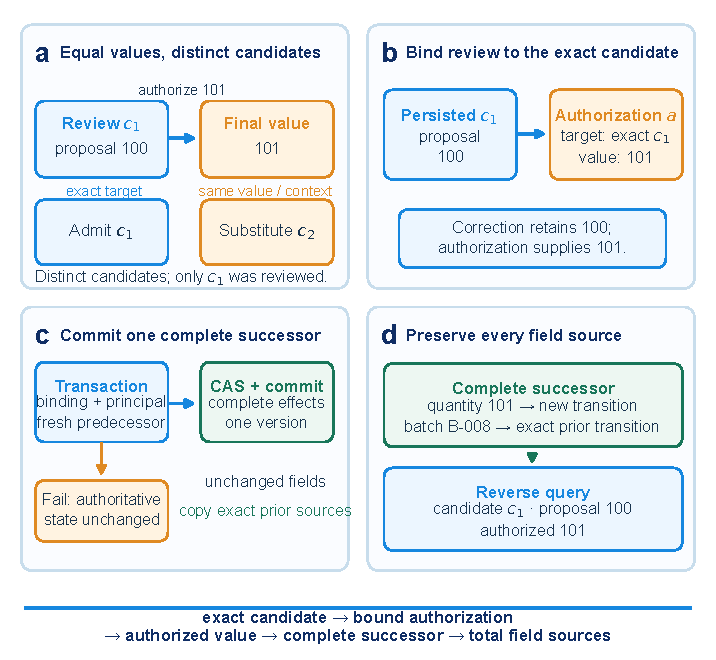
\includegraphics[width=0.975\textwidth]{Fig1.pdf}
\caption{The admission relation preserves both the reviewed instance and the original proposal through Correction. (a) Equal-valued candidates remain distinct authorization targets; (b) the authorized correction retains the proposal; (c) failed admission leaves authoritative state unchanged; (d) changed and unchanged fields retain their respective sources. Values illustrate a constructed example. Diagram preparation assisted by OpenAI Codex; image-generation prototype use is disclosed in Statements and Declarations}
\label{fig:admission-workflow}
\end{figure}
